
\documentclass[12pt,letterpaper]{report}
\usepackage[margin=1in]{geometry}
\usepackage{graphicx}
\usepackage{amsmath}
\usepackage[font=small,labelfont=bf]{caption}
\usepackage[justification=centering]{caption}
\usepackage{tikz}
\usepackage{circuitikz}
\usepackage{siunitx}
\newlength \figwidth
\setlength \figwidth {0.75\linewidth}

\begin{document}

\title{E153 Laboratory Assignment \#2}
\author{Courtney Keeler and Stephen Pinto\\
Harvey Mudd College}
\date{September 30, 2013}
\maketitle

\section*{List of Materials}
\begin{itemize}
	\item Tektronix 2212 Oscilloscope
	\item Pomona 4550B (10X probe)
	\item Elenco LCM-1950 Multimeter
	\item Pre-built mystery circuits
\end{itemize}

\section*{Purpose}
The purpose of this lab is to apply the models for a BNC cable and 10X probe developed in lab 1 by using the two probes to determine the output characteristics of two "mystery circuits."

\section*{Mystery Circuit}
\subsection*{Procedure}

\begin{enumerate}
\item View the output waveform of circuit A using the Tektronix 2212 Oscilloscope and BNC cable
\item Repeat the previous step using the 10X probe
\item Repeat the two previous steps for circuit B
\end{enumerate}

\subsection*{Results}

\begin{figure}
\centering
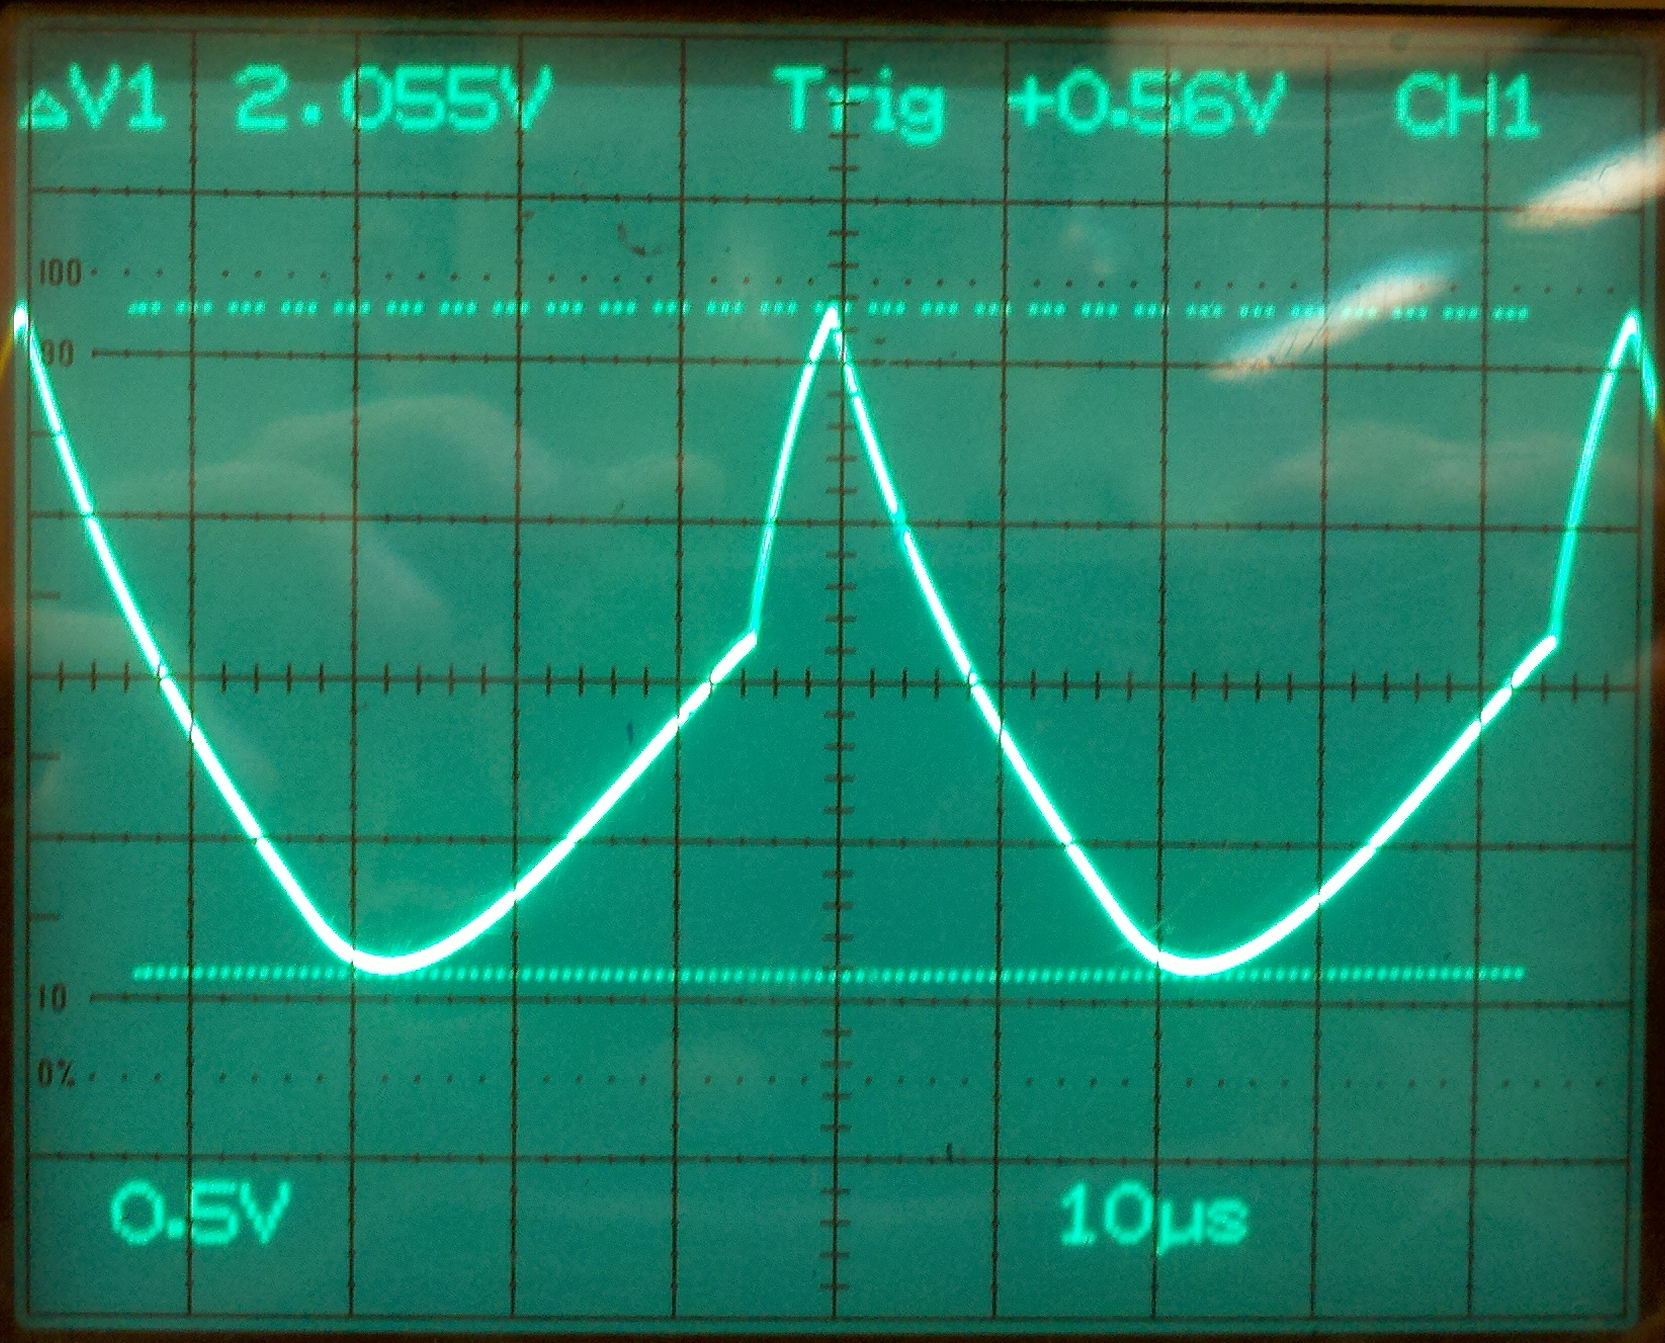
\includegraphics[width=\figwidth, keepaspectratio=true]{lab2/lab2_images/BNC_CircuitA.png}
\caption{Output waveform of circuit A, measured using the BNC cable and oscilloscope.}
\label{fig:bnc_circuit_A}
\end{figure}

\begin{figure}
\centering
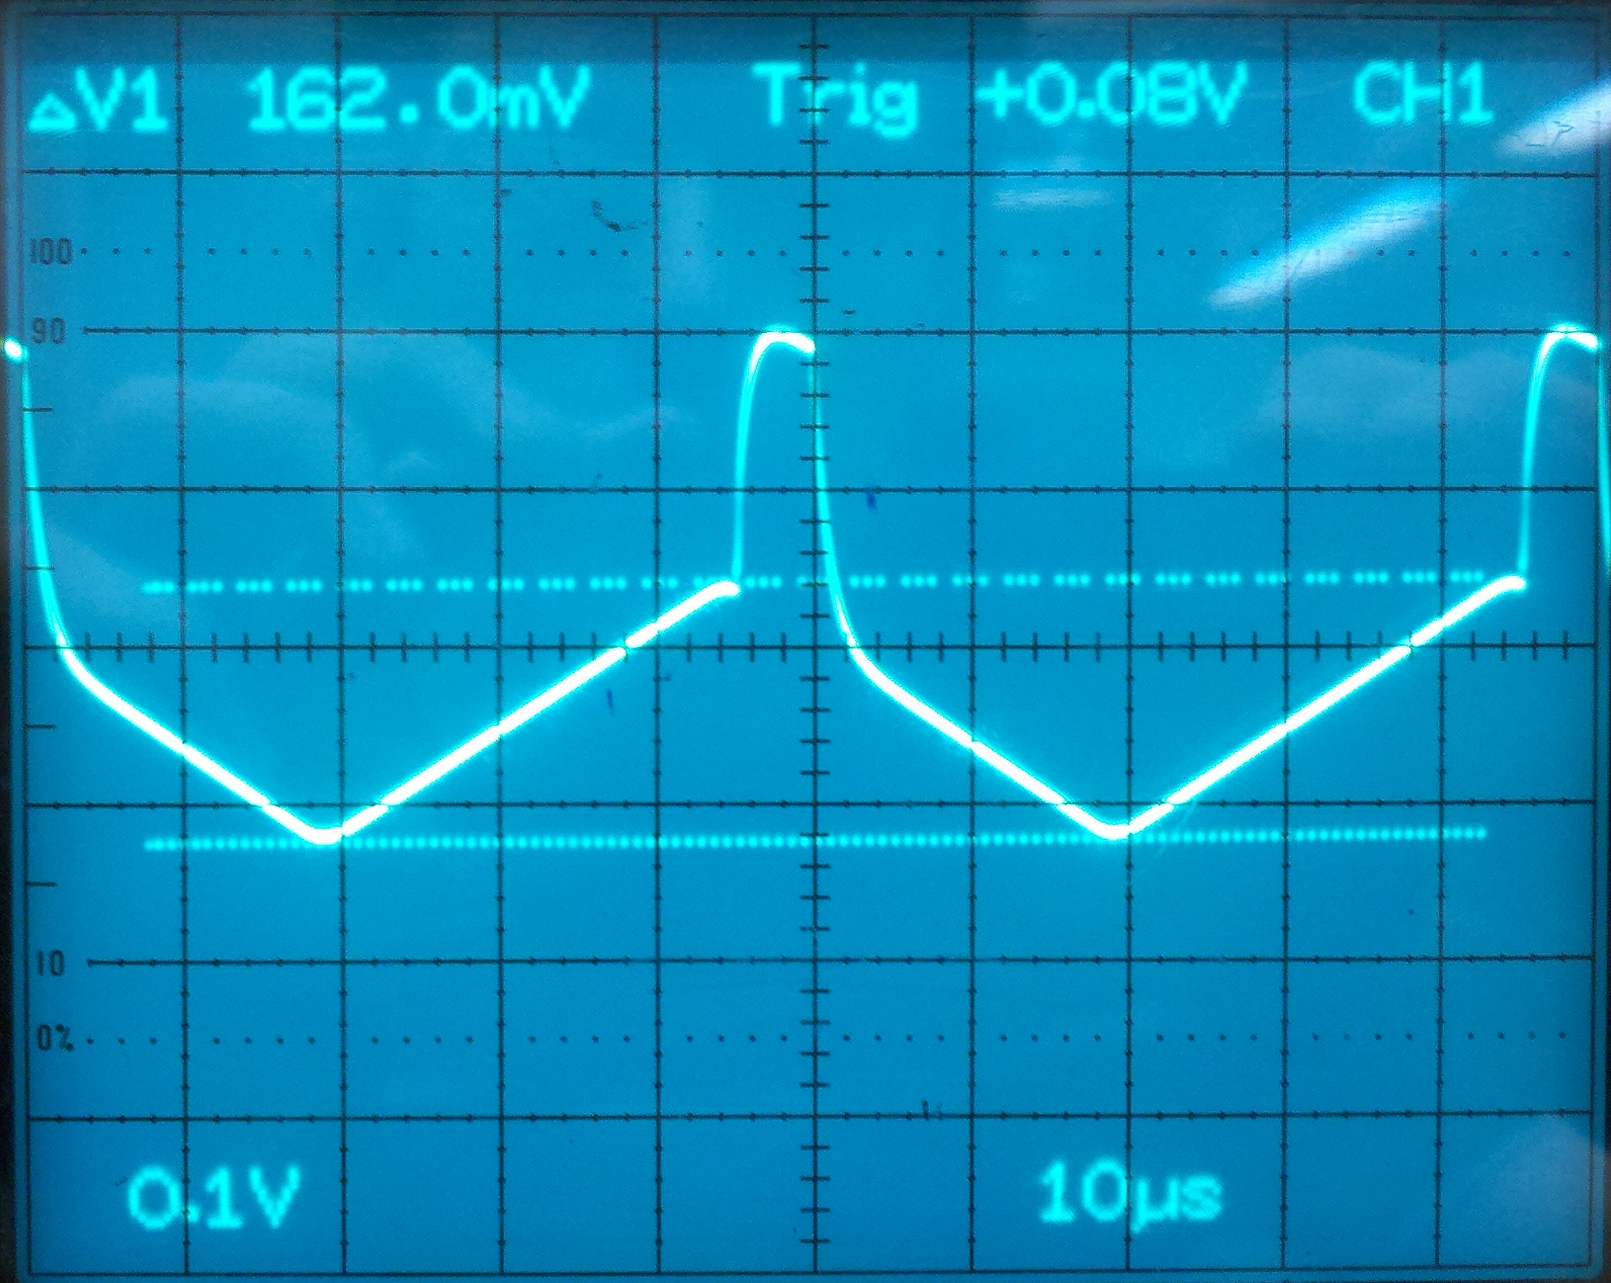
\includegraphics[width=\figwidth, keepaspectratio=true]{lab2/lab2_images/10x_CircuitA_2.png}
\caption{Output waveform of circuit A, measured using the 10X probe and oscilloscope.}
\label{fig:10x_circuit_A}
\end{figure}

\begin{figure}
\centering
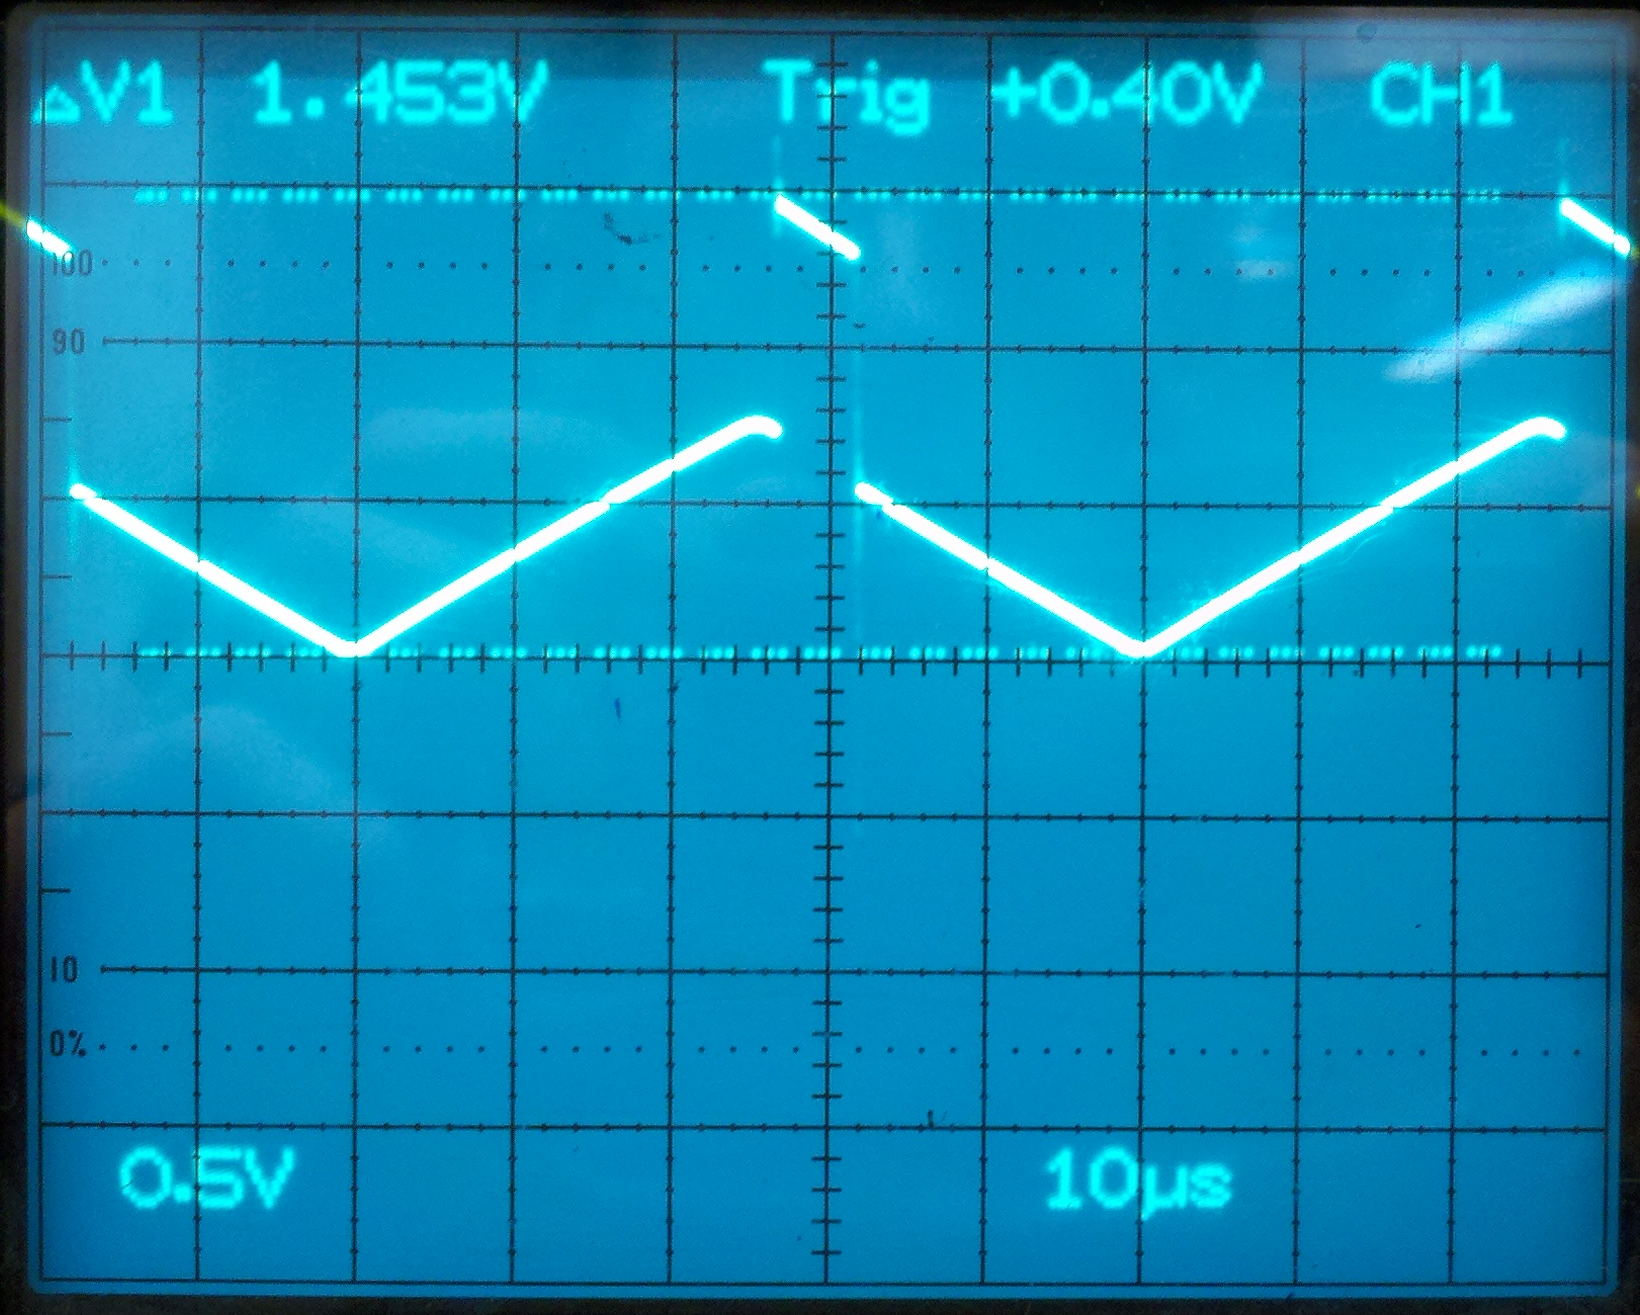
\includegraphics[width=\figwidth, keepaspectratio=true]{lab2/lab2_images/BNC_CircuitB.png}
\caption{Output waveform of circuit B, measured using the BNC cable and oscilloscope.}
\label{fig:bnc_circuit_B}
\end{figure}

\begin{figure}
\centering
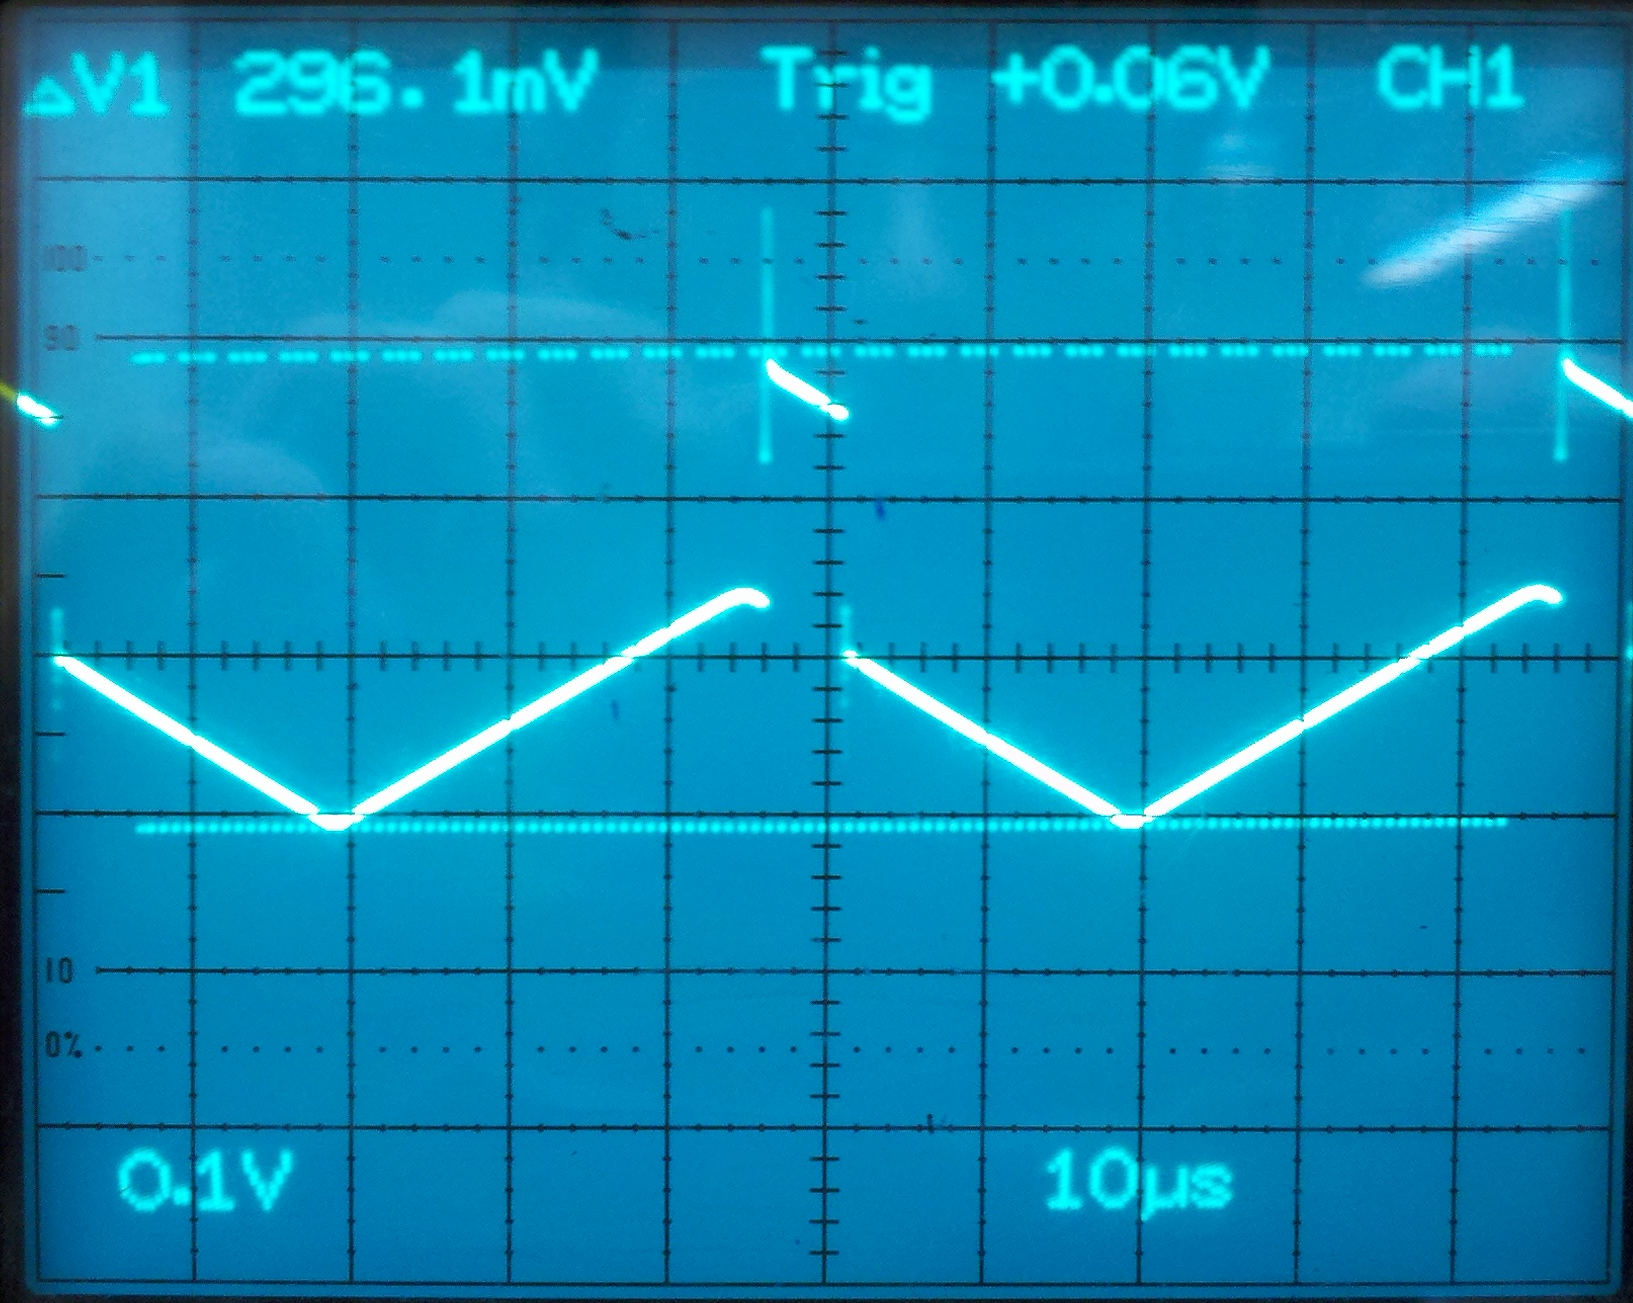
\includegraphics[width=\figwidth, keepaspectratio=true]{lab2/lab2_images/10x_CircuitB.png}
\caption{Output waveform of circuit B, measured using the 10X probe and oscilloscope.}
\label{fig:10x_circuit_B}
\end{figure}

The fundamental frequency of the waveform shown in Figures \ref{fig:bnc_circuit_A} through \ref{fig:10x_circuit_B} is 20.33 kHz. The peak to peak voltage of the triangle wave components for the four waveforms are summarized in Table \ref{table:vpp}.

\begin{table}[ht]
\caption{$\text{V}_{\text{pp}}$ of Triangle Waves} % title of Table
\centering 
    \begin{tabular}{| c | c | c |}
    \hline  
    Circuit & Measuring Device & $\text{V}_{\text{pp}}$ \\
    \hline
    A & BNC & 1.16 V \\
    A & 10X Probe & 162 mV \\
    B & BNC & 1.453 V \\
    B & 10X Probe & 296.1 mV \\
    \hline
    \end{tabular}
    \label{table:vpp}
\end{table}

\section*{Analysis}

\subsection*{Capacitive vs. Resistive}
As described in the lab description provided in class, one of the mystery circuits has only an output resistance and the other has only an output capacitance. To determine which circuit is which, we compared the measurements of the two circuits from the 10x probe with those of the BNC - treating the 10x probe measurements to be the true output and the BNC measurements to be an affected output. As learned in the first lab, the BNC cable is only a capacitor between signal and GND. Meaning for the purely resistive mystery circuit, the overall circuit, including the BNC probe, is a low pass filter. Whereas for the purely capacitive mystery circuit, the overall circuit is simply two capacitors in series with the function generator. Meaning the BNC measurements for the resistive circuit should exhibit filtering effects (namely the input signal's shape should not be fully intact) when compared to the corresponding 10x probe results, while the BNC measurements for the capacitive circuit should only exhibit reduced amplitudes and nothing more (as if it were going through a voltage divider) when compared to the 10x probe results. Figure x, the BNC results of circuit A, show significant filtering effects when compared with Figure y, the 10x results of circuit A. Because of this, we determined that circuit A is the resistive circuit. Similarly, the signals in figure a and b, the results for circuit B, show the exact same waveform just with different amplitudes. As such, we determined that circuit B is the capacitive circuit.


\subsection*{Calculations}

\subsubsection*{Circuit B}
Figure 
%\ref{BNC_circuit_B}
shows the entire circuit for the BNC cable and mystery circuit. However,
we can ignore the resistive elements of the circuits because we know the fundamental frequency of the mystery circuits is 20.33 kHz, which is much greater than 1 kHz, the frequency at which the contribution from resistive and reactive elements are roughly the same. At frequencies higher than 1 kHz, the effects of the resistive elements are negligible. This simplifies the circuit into: an unknown capacitor in series with the BNC capacitor and scope capacitor in parallel. These values were measured following the Lab \# procedure and found to be:
$$
C_{\text{known}} = (C_{ \text{BNC}} | C_{\text{scope}}) = (122 \text{pF} | 20 \text{pF}) = 142 \text{pF}
$$
From this information, we can write the frequency response of the mystery circuit B in terms of the unknown impedance $Z_{\text{unknown}}$ and the known impedance calculated above.
$$
H(jw) = \frac{1}{1+\frac{C_{\text{unknown}}}{C_{\text{known}}}} = \frac{1}{1+\frac{C_{\text{unknown}}}{142 \text{pF}}}
$$
We know that the magnitude of the frequency response of the entire mystery circuit B must be equal to the ratio of the triangle wave peak to peak voltage measured with the BNC cable to the triangle wave peak to peak voltage measured with the 10X probe. This we know because we assume the value of the peak to peak voltage of the triangle wave of circuit B measured by the 10X probe multiplied by ten will be the true output without any effect from measuring devices (The value of ten was calculated in Lab \#1). Since the two capacitors in series are effectively acting as a voltage divider, by measuring the gain between the voltage in (which we assume to be the output voltage measured with the 10X probe) and the voltage out (which will be the output voltage measured with the BNC cable), we can calculate the value of the capacitor that would have caused such a gain.
$$
H(jw) = \frac{1}{1+(\frac{C_{\text{unknown}}}{142 \text{pF}})} = \frac{1.453 \text{V}}{10(.2961\text{V})}
$$
$$
C_{\text{unknown}} = 147 \text{pF}
$$

\subsection*{Mystery Circuit Models}
\begin{center}
\begin{circuitikz} \draw
 (0,0) to[sinusoidal voltage source] (0,2)
 (0,0) to[short, -o] (2,0)
 (0,2) to[R=$\SI{100}{\ohm}$, -o] (2,2)
;\end{circuitikz} \\
\textbf{Mystery Circuit A}

\vspace{2cm}

\begin{circuitikz} \draw
 (0,0) to[sinusoidal voltage source] (0,2)
 (0,0) to[short, -o] (2,0)
 (0,2) to[C=$\SI{100}{\pico\farad}$, -o] (2,2)
;\end{circuitikz} \\
\textbf{Mystery Circuit B}
\end{center}

\end{document}